\documentclass[12pt, onside]{article}

\usepackage{fontspec,unicode-math} % Required for using utf8 characters in math mode
\usepackage{parskip}% Extra interlining
\usepackage[margin=0.8in]{geometry}    % Margins
\usepackage[spanish]{babel}
\usepackage{hyperref}
\usepackage{xcolor}
\usepackage{graphicx}
\usepackage[binary-units=true]{siunitx}
\usepackage{multirow}
\usepackage{mathtools}
\usepackage{array}
\usepackage{physics}
\usepackage{cleveref}
\usepackage[toc,page]{appendix}


% Header and Footer
\usepackage{fancyhdr}
\setlength\headheight{30pt}
\pagestyle{fancy}
\renewcommand{\headrulewidth}{0.4pt}
\fancyhead{}
\fancyhead[L]{
    \textbf{Numerical implementation of the two-body problem}
}
\fancyhead[R]{
    Emilio Domínguez Sánchez
}
\fancyfoot{}
\fancyfoot[C]{\thepage}

% Code Listings Configuration File

\usepackage{listings}
% \renewcommand{\lstlistingname}{Código}
\crefname{lstlisting}{listing}{listings}
\Crefname{lstlisting}{Listing}{Listings}
% \renewcommand{\lstlistlistingname}{Índice de códigos}


\definecolor{background}{rgb}{0.99,0.99,0.99}
\definecolor{mygreen}{rgb}{0.1,0.6,0.1}
\definecolor{mygray}{rgb}{0.5,0.5,0.5}
\definecolor{mymauve}{rgb}{0.58,0,0.82}

\definecolor{codeback}{rgb}{0.85,0,0.85}

\lstset{ 
  title=File \lstname,          % show the filename of files included with \lstinputlisting; also try caption instead of title
  caption=Fichero \texttt{\lstname},
  captionpos=t,                    % sets the caption-position (b/t)
  frame=TBLR,      	               % adds a frame around the code
  rulecolor=\color{black},         % if not set, the frame-color may be changed on line-breaks within not-black text (e.g. comments (green here))
  numbers=left,                    % where to put the line-numbers; possible values are (none, left, right)
  numbersep=10pt,                  % how far the line-numbers are from the code
  stepnumber=0,                    % the step between two line-numbers. If it's 1, each line will be numbered
  backgroundcolor=\color{background},
  numberstyle=\small\color{mygray},% the style that is used for the line-numbers
  basicstyle=\scriptsize\selectfont, % the size/type of the fonts that are used for the code
  keywordstyle=\color{mygreen},       % keyword style
  commentstyle=\color{blue},    % comment style
  stringstyle=\color{mymauve},     % string literal style
  breakatwhitespace=false,         % sets if automatic breaks should only happen at whitespace
  breaklines=true,                 % sets automatic line breaking
  keepspaces=true,                 % keeps spaces in text, useful for keeping indentation of code (possibly needs columns=flexible)
  showstringspaces=false,          % underline spaces within strings only
  showspaces=false,                % show spaces everywhere adding particular underscores; it overrides 'showstringspaces'
  showtabs=false,                  % show tabs within strings adding particular underscores
  tabsize=2,	                   % sets default tabsize to 2 spaces
  language=Matlab,                    % the language of the code
  morekeywords={two_bodies},            % if you want to add more keywords to the set
  deletekeywords={},            % if you want to delete keywords from the given language
  % escapeinside={----}{----},          % if you want to add LaTeX within your code
  extendedchars=true,              % lets you use non-ASCII characters; for 8-bits encodings only, does not work with UTF-8
  literate=
  {á}{{\'a}}1 {é}{{\'e}}1 {í}{{\'i}}1 {ó}{{\'o}}1 {ú}{{\'u}}1
  {Á}{{\'A}}1 {É}{{\'E}}1 {Í}{{\'I}}1 {Ó}{{\'O}}1 {Ú}{{\'U}}1
  {à}{{\`a}}1 {è}{{\`e}}1 {ì}{{\`i}}1 {ò}{{\`o}}1 {ù}{{\`u}}1
  {À}{{\`A}}1 {È}{{\'E}}1 {Ì}{{\`I}}1 {Ò}{{\`O}}1 {Ù}{{\`U}}1
  {ä}{{\"a}}1 {ë}{{\"e}}1 {ï}{{\"i}}1 {ö}{{\"o}}1 {ü}{{\"u}}1
  {Ä}{{\"A}}1 {Ë}{{\"E}}1 {Ï}{{\"I}}1 {Ö}{{\"O}}1 {Ü}{{\"U}}1
  {â}{{\^a}}1 {ê}{{\^e}}1 {î}{{\^i}}1 {ô}{{\^o}}1 {û}{{\^u}}1
  {Â}{{\^A}}1 {Ê}{{\^E}}1 {Î}{{\^I}}1 {Ô}{{\^O}}1 {Û}{{\^U}}1
  {œ}{{\oe}}1 {Œ}{{\OE}}1 {æ}{{\ae}}1 {Æ}{{\AE}}1 {ß}{{\ss}}1
  {ű}{{\H{u}}}1 {Ű}{{\H{U}}}1 {ő}{{\H{o}}}1 {Ő}{{\H{O}}}1
  {ç}{{\c c}}1 {Ç}{{\c C}}1 {ø}{{\o}}1 {å}{{\r a}}1 {Å}{{\r A}}1
  {€}{{\euro}}1 {£}{{\pounds}}1 {«}{{\guillemotleft}}1
  {»}{{\guillemotright}}1 {ñ}{{\~n}}1 {Ñ}{{\~N}}1 {¿}{{?`}}1
}



\newcommand{\R}{{\mathbb{R}}}
% \renewcommand{\dv}{\prime}
\newcommand{\ddv}{\dprime}
\newcommand{\inner}[2]{\left\langle #1, \; #2 \right\rangle}
\newcommand{\vr}{{\vb{r}}}
\newcommand{\vx}{{\vb{x}}}
\newcommand{\CM}{{\operatorname{CM}}}

\begin{document}
\begin{titlepage}
    \begin{center}
        \vspace*{1cm}
        
        \Huge \textbf{Two-Body Problem}
        
        \vspace{0.5cm}
        \LARGE Analysis and Implementation
        
        \vspace{0.5cm}
        
        \Large Assignment for \\ Métodos Numéricos de las Ecuaciones Diferenciales
        
        \vspace{0.5cm}
   		
        \vfill
        
        %Obor XY
        \vspace{0.8cm}
        \Large
            \begin{flushright}
              	\begin{tabular}{lr}
                  Author: & Emilio Domínguez Sánchez\\
                  Due Date: & 7th of November of 2020\\
                \end{tabular}
            \end{flushright}
        \vspace{0.5cm}
        
    \end{center}
\end{titlepage}

\newpage
\tableofcontents
\newpage

\section{Introduction}

    The two-body problem is the study of the motion of two bodies (particles)
that only interact between them.
The problem is usually encountered in astronomy because
it is typical to encounter two astronomical objects
that are widely separated from other objects,
making it possible to ignore their gravitational forces.

    In this paper, we study the earth's and sun's mutual gravitational interaction,
reduce it to a simpler problem
and solve it numerically using fixed step ordinary differential equations (ODEs) solvers.

\section{Problem description}

    Consider two isolated particles of constant mass $M_1$ and $M_2$ respectively.
If we only consider the gravitational force,
the equation for universal gravitation states that both that
both objects are attracted by a force

\begin{equation*}
    F = G\frac{M_1M_2}{\norm{\vr_2-\vr_1}^2},
\end{equation*}

\noindent
where $r_1$ and $r_2$ are the positions of both objects.

    Hence, it is possible to write the acceleration both objects suffer and
to write a differential equation that expresses their motion
(given some initial conditions for position and speed).

\subsection{Initial Value Problem}

$\vr_1(t_0)$, $\vr_2(t_0)$, $\dv{\vr_1}{t}(t_0)$ and $\dv{\vr_2}{t}(t_0)$ shall be known
and the rest of the motion is determined by the equations

\begin{equation*}
    \begin{dcases}
        \dv[2]{\vr_1}{t} = \frac{F}{M_1} \; \frac{\vr_2-\vr_1}{\norm{\vr_2-\vr_1}} \\
        \dv[2]{\vr_2}{t} = \frac{F}{M_2} \; \frac{\vr_1-\vr_2}{\norm{\vr_1-\vr_2}}
    \end{dcases}.
\end{equation*}

    This problem has to be reduced to the initial value problem

\begin{gather*}
    \vx(t_0) = \mqty(
        \vr_1(t_0) &
        \vr_2(t_0) &
        \dv{\vr_1}{t}\, (t_0) &
        \dv{\vr_2}{t}\, (t_0)
    ) \\
    \vx = \mqty(
        \vx_3 &
        \vx_4 &
        \frac{GM_2}{\norm{\vx_2-\vx_1}^3} \; (\vx_2-\vx_1) &
        \frac{GM_1}{\norm{\vx_2-\vx_1}^3} \; (\vx_1-\vx_2)
    ),
\end{gather*}

\noindent
which, if we are stuyding a motion in $\R^3$, is a problem of dimension $12$.
Fortunately, we can further study the problem to simplify it to dimension $4$.

\subsection{Simplification by symmetry}

    The problem we are studying is inherently symmetric.
The force applied to each body is the same and depends on the distance between both bodies,
not on their position.
And the direction depends on their relative position,
which also expresses their distance.
That means that we can write the motion in terms of the relative distance, $\vr_2-\vr_1$,
instead of both $\vr_1$ and $\vr_2$,
reducing the number of variables of the system in half.

\begin{gather*}
    \vr = \vr_2-\vr_1 \\
    \dv[2]{\vr}{t} =
    \dv[2]{\vr_2}{t} - \dv[2]{\vr_1}{t} =
    \frac{GM_1}{\norm{\vr}^3}(-\vr) - \frac{GM_2}{\norm{\vr}^3}\vr =
    - \frac{G(M_1+M_2)}{\norm{\vr}^3}\vr
\end{gather*}

    This would leave us with a system of dimension $6$,
but we would only solve the problem for the relative position.
We need a way to reconstruct the original solution,
of which we only know that $\vr_2(t)t-\vr_1(t) = \vr(t)$.

\subsection{Reconstruction with respect to the center of mass}

    The center of mass of a set of points is an hypothetical point
that represents the position of a particle that would encompass all those points.
That is, the point where the mass distributed along those objects sums zero.
In our problem, the center of mass is at $\vr_{\CM} = \frac{M_1\vr_1 + M_2\vr_2}{M_1+M_2}$.

    The interesting thing is that

\begin{equation*}
    \dv[2]{vr_{\CM}}{t} =
    \frac{1}{M_1+M_2}\qty(M_1\dv[2]{\vr_1}{t} + M_2\dv[2]{\vr_2}{t}) =
    0.
\end{equation*}

\noindent
And because the center of mass is stationary or moves at constant speed,
it serves as a secondary inertial frame of reference\footnotemark.
In this frame of reference $M_1\vr_1 + M_2\vr_2 = 0$,
which makes it possible to obtain the values of $\vr_1$ and $\vr_2$ given $\vr$.

\footnotetext{Comprehensive information about what is a inertial frame of reference
can be found in \href{https://en.wikipedia.org/wiki/Inertial_frame_of_reference}{Wikipedia}.
But basically, it is a reference where newton's law has the traditional form
$\vb{F} = m\vb{a}$
and the formulas written until now hold.}

\begin{equation*}
    \begin{dcases}
        \vr = \vr_2-\vr_1 \\
        0 = M_1\vr_1 + M_2\vr_2
    \end{dcases}
    \implies
    \begin{dcases}
        \vr_1 = \frac{-M_2}{M_1+M_2}\vr \\
        \vr_2 = \frac{M_1}{M_1+M_2}\vr
    \end{dcases}
\end{equation*}

\subsection{Simplification by motion}

    This last simplification will reduce our $6$ dimensional problem to
a problem of dimension $4$.
The observation required now is that the movement $\vr$ is planar because its torsion is $0$.

\begin{equation*}
    τ_\vr =
    \frac{\det\mqty(\vr & \dv{\vr}{t} & \dv[2]{\vr}{t})}
        {\norm{\dv{\vr}{t} \times \dv[2]{\vr}{t}}^2} =
    \qty(\text{$\vr$ collinear with $\dv[2]{\vr}{t}$}) =
    0.
\end{equation*}

\noindent
(\textbf{Note:} Those more familiar with physics concepts will prefer to study
the angular movement of the system, which is constant, than the torsion.)

    As a result, we can choose the frame of reference centered on the center of mass for which
the movement is contained in the plane $z = 0$.

\section{Sun-Earth Problem}

    The rest of the paper in focused on solving the two-body problem
for the sun ($\vr_1$) and the earth ($\vr_2$).
As discussed, we will choose the frame of reference given by the center of mass
and such that the movement is contained in the plane $z = 0$.
That is, we will work on $\R^2$.

    It is well known that the earth describes an elliptical motion
where the sun is a focus point.
Meaning $\vr$ periodic with periodicity one year.
Our objective is to calculate the time lapse that corresponds to a year.

\subsection{Obtaining trusted data}

    To solve our system of equations we need both parametrical data;
like the constant $G$ and the masses of the earth and the sun;
as well as initial conditions for $\vr$;
the relative position of both bodies and
the speeed of the relative position at a given time.
The National Aeronautics and Space Administration (NASA)
provides accurated data we can use\footnotemark.

\footnotetext{For example, we can consult
\href{https://nssdc.gsfc.nasa.gov/planetary/factsheet/earthfact.html}{the Earth's fact sheet}.}

    However, obtaining the values of $\vr(t_0)$ and $\dv{\vr}{t}{(t_0)}$
is more complicated than it seems.
The points at which the Earth is the farthest and closest from or to the sun
are called aphelium and periheliom.
NASA provides values for both distances and the speed at those moments (as a scalar).
But how do we know what is the angle between the position and the speed?
Well, at a local maximum (resp. minimum) in the distance,
the derivative of that distance,
which is proportional to the escalar product of speed and position,
has to be zero,
meaning that they are orthogonal.
In mathematical formulas:

\begin{equation*}
    \begin{dcases}
        \operatorname{distance} = \frac{\vr}{\norm{\vr}} \\
        \dv{\frac{\vr}{\norm{\vr}}}{t} = \frac{\inner{\dv{\vr}{t}}{\vr}}{\norm{\vr}}
    \end{dcases}
    \implies
    \qty[ \frac{\vr}{\norm{\vr}} \text{is maximum} \iff \dv{\vr}{t} \perp \vr ].
\end{equation*}

    Knowing that, we can set our initial point as
$\vr(t_0) = (\operatorname{max\ distance}, 0)$
and the velocity as
$\dv{\vr}{t}(t_0) = (0, \operatorname{speed\ at\ max\ distance})$.

\subsection{Initial Value Problem}

\begin{center}
    \begin{tabular}{m{5cm} c}
        \textbf{NASA Public Data} &
        \begin{tabular}{p{5.5cm} | m{3cm}}
            \textit{Magnitude} & \textit{Measure} \\
            \hline \hline \\
            Constant $G$ & $\SI[per-mode=fraction]{6.67430}{\meter^3\per{\kg\second^2}}$ \\
            Mass Sun ($M_1$) & $\SI{1.9885e30}{\kg}$ \\
            Mass Earth ($M_2$) & $\SI{5.9724e24}{\kg}$ \\
            Maximum distance between the earth and the sun ($x_0$) & $\SI{1.521e8}{\km}$ \\
            Speed at maximum distance between the earth and the sun ($v_0$) &
                $\SI[per-mode=fraction]{2.929}{\km\per\second}$ \\
            Minimum distance between the earth and the sun & $\SI{1.4709e8}{\km}$ \\
            Speed at minimum distance between the earth and the sun &
                $\SI[per-mode=fraction]{3.029}{\km\per\second}$ \\
            Earth's orbit year & $\SI{365.242}{\day}$ \\
        \end{tabular}
        \vspace{1cm} \\

        \textbf{Formulation} &
        $
        \begin{gathered}
            \vx(0) = \mqty(x_0 & 0 & 0 & v_0) \\
            \dv{\vx}{t} = \mqty(
                \vx_3 &
                \vx_4 &
                -\frac{G(M_1+M_2)}{\norm{\smqty(\vx_1 & \vx_2)}^3}\vx_1 &
                -\frac{G(M_1+M_2)}{\norm{\smqty(\vx_1 & \vx_2)}^3}\vx_2
            )
        \end{gathered}
        $
    \end{tabular}
\end{center}

\section{Implementation}

    To solve our problem we will implement some fixed step methods and compare their results.
The language of choice has been \href{https://julialang.org/}{Julia}.

\subsection{Choice of units}

    Real numbers are stored in scientific notation with a fixed number of bits in computers.
This means that independently of the units we use to measure a number,
we obtain roughly the same precision and only the exponent changes\footnotemark.
That independency in the relative error is maintained across multiplications and divisions,
where the significands and exponents are multiplied independently.
However, it is lost when performing additions and substractions.
If we add a very small number to a very big number,
we loose the information of the smallest bits which do not fit in the significand.
Therefore, choosing units that make all numbers of similar magnitude
can make the program more accurate.

\footnotetext{I say roughly because if the factor is not a power of two,
then the significand of a particular number changes and
it could be better or worse represented.
However, this is not traceable for all operations involved in an algorithm.}

    For that reason, in the code,
length is measured in $\si{\km}$,
mass is measured in $\SI{1e27}{\kg}$ and
time is measured in hours.

\subsection{Methods}

    We compare $4$ different fixed step methods to solve ODEs.
The traditional Euler's method,
wich requires one evaluation of the derivative function and
guarantees an error $\mathcal{O}(\operatorname{step})$;
an improved version of Euler's method,
that performs two evaluations and guarantees an error of $\mathcal{O}(\operatorname{step}^2)$;
Heum's method, with two evaluations and an error of $\mathcal{O}(\operatorname{step}^2)$; and
the Runge-Kutta $4$ method,
with $4$ evaluations and an error of $\mathcal{O}(\operatorname{step}^4)$.
The source code can be found in \cref{lst:fixed-step-methods}.

\section{Relevant measures}

    Having procedures to compute solutions,
we now investigate how to obtain sensible data from the output.

\subsection{Stop condition}

    In order to obtain the year time lapse or the calculated minimum distance,
we need to be able to stop the procedure at specific moments.
In our case, we are interested in stopping the movements after completing a whole loop
or half a loop (moment that corresponds to the minimum distance in the ellipse).

\begin{lstlisting}[caption=Stop conditions for the code]
function full_turn(t, x)
    p2 = x[length(x)-1][1:2]
    p1 = x[length(x)][1:2]
    return p2[2] < 0 && p1[2] >= 0
end

function half_turn(t, x)
    p2 = x[length(x)-1][1:2]
    p1 = x[length(x)][1:2]
    return p2[2] > 0 && p1[2] <= 0
end
\end{lstlisting}

\subsection{Hermite Interpolation: Adjusting the last point}

    Another problem is aproximating the point we want as much as possible.
Even if we stop the method as close as possible to that point (with the current step),
we cannot guarantee that the last point will be close enough to it.
One of the options, and the one we chose,
was to interpolate that point using some of the last values.
Therefore, we implemented hermite interpolation.

    Of the aphelium and periheliom we know that their second coordinate is $0$.
Therefore, the interpolation was performed
using the last values for the second coordinate and
evaluating the resulting polynomial at $0$.
Note that in our problem, at the aphelium and periheliom,
$\vr_x$ can be written as a function of $\vr_y$ for some neighborhood,
because the derivative has a non zero second component.
(Indeed, the solution is an ellipse. Thus the neighborhood is very big.)
This supports the fact that $\vr_x$ can be interpolated using the values of $\vr_y$.
%TODO foto?

\subsection{The earth's year and the periheliom}

    Stopping the procedure after completing a turn and
using hermite interpolation with the closest $5$ points
we were able to interpolate the aphelium (after a whole turn)
and the periheliom (after half a turn).

    For each method, we obtained
the year length, the aphelium after a whole turn and the periheliom.
We compared (\cref{lst:script}) the aphelium with the starting point and
the distance in the periheliom and the year with the data provided by NASA.

\begin{lstlisting}{caption=Execution results with step of size $1$}
two_bodies> 
	Method euler_step
	Closing Error: 0.08381386440137123
	Year: 367.67506150760715
	Year Error(NASA): 2.4330615076071354
	Periheliom: 147.72425053797423
	Periheliom Error(NASA): 0.6342505379742249

two_bodies> 
	Method mod_euler_step
	Closing Error: 0.020284135563232587
	Year: 365.2003179673815
	Year Error(NASA): 0.04168203261849612
	Periheliom: 147.06963706885708
	Periheliom Error(NASA): 0.020362931142926755

two_bodies> 
	Method heum_step
	Closing Error: 0.020504951954471655
	Year: 365.20023071081033
	Year Error(NASA): 0.0417692891896877
	Periheliom: 147.06960229925187
	Periheliom Error(NASA): 0.020397700748134184

two_bodies> 
	Method RK4_step
	Closing Error: 0.02091759638215969
	Year: 365.2000676518665
	Year Error(NASA): 0.0419323481335141
	Periheliom: 147.069525352274
	Periheliom Error(NASA): 0.02047464772599028
\end{lstlisting}

\section{Study of the error}

    The values provided by NASA are not based in this simplified model,
but on empirical measurements.
This means that reducing the step of the methods does not make them converge to them,
but to the theoretical measures.
Hence, they are practical for testing whether a method is well implemented,
but they cannot be used to compare the different methods.

    The closing error ought to be better aproximation in our case,
because it only depends on the theoretical solution.
But it is not enough alone,
as we do not know how much the orbit differs from the solution midways.
In the initial results, we see that
the closing error is notably higher in the Euler method, which is only
$\mathcal{O}(\operatorname{step})$.
On the other hand, we don't obtain more precision using the Runge-Kutta method,
as one could expect.
Could it be that it were not so well suited for this problem?

\subsection{Explanation of the error}

    We have seen we could approximate the solution very well,
but the question as to why the Runge-Kutta is not better still remains.
What is more, executing the code with smaller steps does not modify the results,
the $\mathcal{O}(\operatorname{step}^2)$ and the $\mathcal{O}(\operatorname{step}^4)$ methods
perform almost the same.
It is true that there are methods to approximate the error with a given step size,
but in this work,
we thought it would be interesting to apply methods specific to this problem.

    The first idea was to see what happened when we increased the size.
Take a look at the \cref{fig:step1,fig:step50,fig:step100,fig:step150}.
The results are obvious.
Even with much higher steps we obtain visually closed orbits for all methods except Euler's.

    In the case of Euler's method, it is only natural that
the orbit is much worse as the step size increases.
Take into account that the orbit of the Earth is almost a circle.
At any point of circunference, an Euler step increases the radius of the movement,
making it bigger and bigger.
The rest of the methods use a combination of tangents that makes the point
traverse along a secant of the circunference,
and that is the reason they perform better with bigger steps.
To prove this statement, consider the Heum's method.
The Heum's method is not symmetric,
in contrast to the modified Euler's method and Runke-Kutta 4,
because one tangent has a factor of $\frac{1}{4}$ and the other of $\frac{3}{4}$.
As a result, it is worse at closing the orbit, as can be seen in \cref{lst:output-step-150}.

    As for the accuracy of the methods,
we use the data to also prove that the fact that the orbit is closed is not enough to prove
a good convergence of the method.
Presumably, because the different errors along the path can cancel one another in the end
but still be present along the curve.
Notice that with the biggest step (\cref{lst:output-step-150}),
the closing error for the improved Euler's method is like that of the Runge-Kutta method,
but the calculus for the year differs in more than $6$ days,
while the difference is $0.04$ days for the Runge-Kutta method.
The conclusion is that the orbit is ``much'' longer than the theoretical orbit,
even though it has a similar deviation from being a closed curve as
the $\mathcal{O}(\operatorname{step}^4)$ method,
which is still close to the theoretical orbit in length.

\begin{figure}[p]
    \centering
    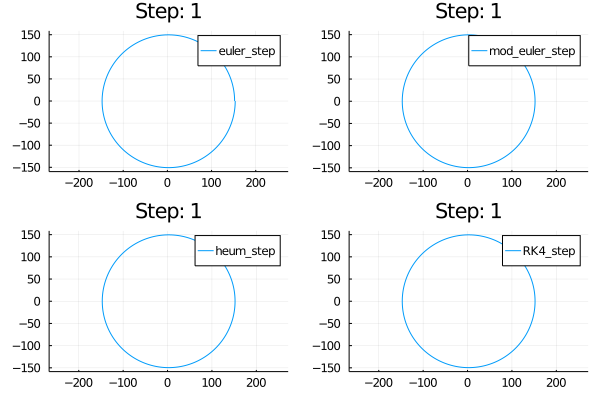
\includegraphics[width=0.8\textwidth]{media/two_bodies_step_1.png}
    \caption{Graphical representation with $\operatorname{step} = 1$}
    \label{fig:step1}
\end{figure}

\begin{figure}[p]
    \centering
    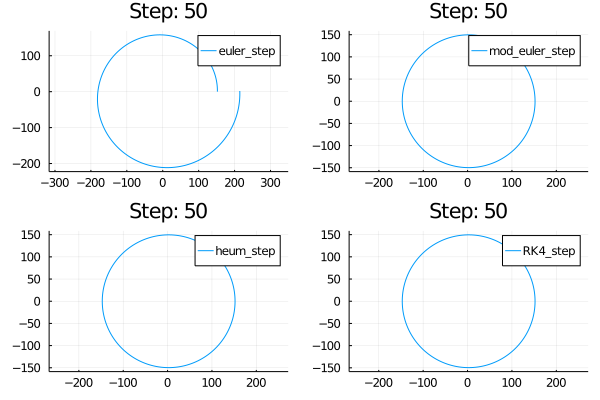
\includegraphics[width=0.8\textwidth]{media/two_bodies_step_50.png}
    \caption{Graphical representation with $\operatorname{step} = 50$}
    \label{fig:step50}
\end{figure}

\begin{figure}[p]
    \centering
    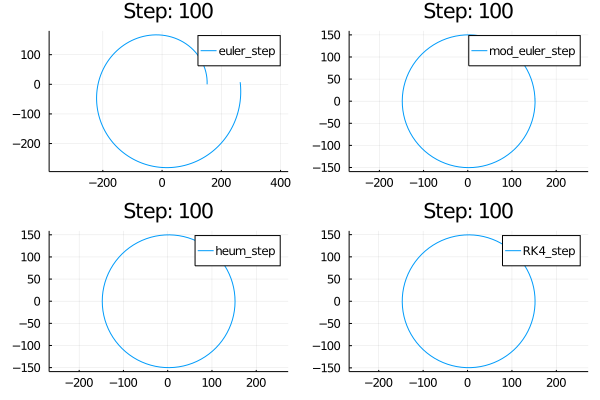
\includegraphics[width=0.8\textwidth]{media/two_bodies_step_100.png}
    \caption{Graphical representation with $\operatorname{step} = 100$}
    \label{fig:step100}
\end{figure}

\begin{figure}[p]
    \centering
    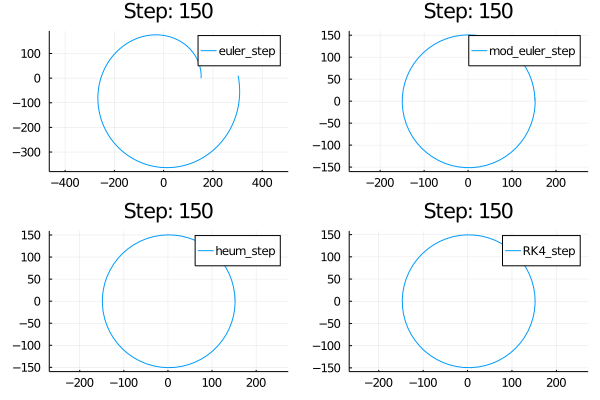
\includegraphics[width=0.8\textwidth]{media/two_bodies_step_150.png}
    \caption{Graphical representation with $\operatorname{step} = 150$}
    \label{fig:step150}
\end{figure}

\section{Conclusions}

    The conclusions to the study of the different numerical methods for this problem are that

\begin{itemize}
    \item The measure of the accuracy of the methods are based on the worst case,
    and some methods can perform reasonably well for particular problems
    with steps manageable by any current computer.

    \item In the absence of an analytical solution,
    it is not enough to test our solution in a particular qualitative measure as
    how the orbit deviates from being closed.
    Although the more qualitative measures we have that assert that
    the computed solution behaves as expected,
    the more confident we can be.

    \item It is important to have methods that can estimate the error of a solution
    without an annalytical solution.
\end{itemize}

Interestingly, the formulas that allow to estimate the error of a solution
also serve as a base to develop adaptative steps methods,
which we will proceed to study in our subject.

\newpage

\begin{appendices}

\section{Julia Code}

\lstinputlisting[label=lst:fixed-step-methods]{src/FixedStepMethods.jl}

\lstinputlisting[label=lst:hermite-inerpolation]{src/Interpolation.jl}

\lstinputlisting[label=lst:script]{scripts/two_bodies.jl}

\section{Methods Output for each step}

\lstinputlisting[label=lst:output-step-1]{outputs/two_bodies_step_1.txt}

\lstinputlisting[label=lst:output-step-50]{outputs/two_bodies_step_50.txt}

\lstinputlisting[label=lst:output-step-100]{outputs/two_bodies_step_100.txt}

\lstinputlisting[label=lst:output-step-150]{outputs/two_bodies_step_150.txt}

\end{appendices}

\end{document}
